\documentclass[12pt, a4paper]{report}

% Encoding and language
\usepackage[utf8]{inputenc}
\usepackage[croatian]{babel}
\usepackage[T1]{fontenc}

% Layout
\usepackage[left=3cm, right=2.5cm, top=2.5cm, bottom=2.5cm]{geometry}
\usepackage{setspace}
\onehalfspacing

% Graphics and figures
\usepackage{graphicx}
\graphicspath{{figures/}}
\usepackage{float}
\usepackage{tikz}

% Math
\usepackage{amsmath}
\usepackage{amssymb}

% Tables
\usepackage{booktabs}
\usepackage{tabularx}

% Code listings
\usepackage{listings}
\usepackage{xcolor}

% References and links
\usepackage{hyperref}
\hypersetup{
    pdftitle={Primjena računalnog vida u sustavima za izbjegavanje sudara kod autonomnih vozila i pametnih sustava asistencije vozaču (ADAS)},
    pdfauthor={Daniel Batinić},
    pdfsubject={Završni rad — Fakultet elektrotehnike i računarstva, Sveučilište u Zagrebu},
    pdfkeywords={ADAS, računalni vid, Canny, detekcija traka, kinematički model, izbjegavanje sudara, autonomna vozila},
    pdfcreator={LaTeX s MiKTeX distribucijom},
    pdfproducer={Daniel Batinić, 2026.},
    colorlinks=true,
    linkcolor=black,
    citecolor=black,
    urlcolor=blue
}
\usepackage[backend=biber, style=ieee]{biblatex}
\addbibresource{references.bib}

% Header/Footer
\usepackage{fancyhdr}
\pagestyle{fancy}
\fancyhf{}
\rhead{\leftmark}
\cfoot{\thepage}

% paddings
\usepackage{titlesec}
\titleformat{\chapter}[hang]{\LARGE\bfseries}{\thechapter.~}{0pt}{}
\titlespacing*{\chapter}{0pt}{-40pt}{20pt}
\titleformat{\section}[hang]{\large\bfseries}{\thesection}{1em}{}
\titleformat{\subsection}[hang]{\normalsize\bfseries}{\thesubsection}{1em}{}

% -----------------------------------------------

\begin{document}

% Title page
\begin{titlepage}
    \begin{tikzpicture}[remember picture, overlay]
        \node[anchor=south east, xshift=-1cm, yshift=0.5cm, font=\tiny\color{gray}]
        at (current page.south east) {v1.0};
    \end{tikzpicture}

    \centering
    
\includegraphics[width=11cm]{figures/FER_logo_3.png}

    \vspace{0.5cm}
    {\large Sveučilište u Zagrebu\par}
    {\Large\bfseries Fakultet elektrotehnike i računarstva\par}

    \vspace{1.5cm}
    {\large Završni rad\par}

    \vspace{2cm}
    {\LARGE\bfseries Primjena računalnog vida u sustavima za izbjegavanje sudara kod autonomnih vozila i pametnih sustava asistencije vozaču (ADAS)\par}

    \vspace{3cm}
    \begin{tabular}{ll}
        \textbf{Autor:}  & Daniel Batinić                   \\[0.5em]
        \textbf{Mentor:} & izv. prof. dr. sc. Daniel Hofman \\
    \end{tabular}

    \vfill
    {\large Zagreb, 2026.\par}
\end{titlepage}

% Rimski brojevi za prednji dio
\pagenumbering{roman}
\setcounter{page}{1}

% Sažetak (HR)
\newpage
\thispagestyle{empty}
\phantomsection
\addcontentsline{toc}{chapter}{Sažetak}
\null\vfill
\begin{center}
    {\Large\bfseries Sažetak\par}
    \vspace{1cm}
    \begin{minipage}{0.6\textwidth}

        Ovdje ide sažetak na hrvatskom jeziku.
    \end{minipage}
\end{center}
\vfill\null

% Abstract (EN)
\newpage
\thispagestyle{empty}
\phantomsection
\addcontentsline{toc}{chapter}{Abstract}
\null\vfill
\begin{center}
    {\Large\bfseries Abstract\par}
    \vspace{1cm}
    \begin{minipage}{0.6\textwidth}

        Here goes the abstract in English.
    \end{minipage}
\end{center}
\vfill\null

% Sadržaj
\newpage
\tableofcontents

% Arapski brojevi od prvog poglavlja
\clearpage
\pagenumbering{arabic}
\setcounter{page}{1}

% Chapters
% !TeX root = ../main.tex
\chapter{Uvod}

Moderni prometni sustavi sve više ovise o sustavima asistencije vozaču (ADAS), čiji je glavni cilj smanjiti učestalost prometnih nesreća i povećati sigurnost svih sudionika u prometu. U tom smislu, računalni vid predstavlja jednu od važnih tehnologija jer omogućuje analizu prometne scene iz izvora video zapisa (kamere) u stvarnom vremenu. S pomoću detekcije prometnih traka, prepoznavanja objekata i procjene rizika sudara, moguće je upozoriti vozača ili aktivirati automatsku reakciju sustava.

Ovaj rad prikazuje razvoj i evoluciju jednog cjelovitog, determinističkog ADAS prototipa temeljenog na klasičnim metodama obrade slike. Sustav je napravljen tako da odvaja glavne korake u predikciji sudara: kontekstnu analizu scene (vidljivost, uvjeti na cesti), detekciju traka, detekciju i praćenje objekata, procjenu rizika sudara te donošenje odluke o upozorenju ili kočenju. Poseban naglasak je stavljen na robusnost sustava tako da isti može raditi za različite scenarije i uvjete.

\section{Motivacija}
Iako su modeli dubokog učenja danas većinski zastupljeni u implementacijama sustava koji koriste neke oblike računalnog vida, njihova primjena često zahtijeva velike količine anotiranih podataka, snažan hardver i složeno održavanje modela. U inženjerskim i edukacijskim scenarijima nerijetko je korisno razviti sustav koji je brz, predvidljiv i računalno učinkovit. Upravo zbog toga motivacija ovog rada je izgraditi ADAS pipeline koji se može analizirati korak po korak, gdje je svaka odluka sustava povezana s mjerljivim parametrima i jasnim pravilima.

Dodatna motivacija proizlazi iz potrebe da se sustav ponaša prilagodljivo ovisno o kontekstu scene. U stvarnim uvjetima vožnje kvaliteta slike, vidljivost traka i stanje podloge mogu se značajno mijenjati. Zbog toga je uveden kontekstno svjestan mehanizam usmjeravanja režima rada (scenario routing) koji dinamički prilagođava način detekcije i kriterije za procjenu rizika.

\section{Ciljevi rada}
Glavni cilj rada je implementirati funkcionalan i modularan ADAS sustav za obradu slika video \textit{stream}-a prometne kamere, analizu scenarija te evaluirati ponašanje samog sustava kroz niz testnih slučajeva. Kako bi se taj cilj ostvario, definirani su sljedeći podciljevi:

\begin{itemize}
    \item projektirati arhitekturu sustava koja jasno odvaja kontekstnu analizu, percepciju, procjenu rizika i korisničko sučelje,
    \item implementirati detekciju prometnih traka i prepreka klasičnim metodama obrade slike,
    \item uvesti metriku rizika sudara (TTC i kombinirani \textit{risk score}) te pravila odlučivanja za akcije upozorenja i kočenja,
    \item omogućiti kontekstno prilagođavanje parametara sustava (npr. degradirani uvjeti, slabije vidljive trake, mokra podloga),
    \item izgraditi alate za pokretanje scenarija, debug prikaz i evaluaciju rezultata,
    \item dokumentirati ograničenja i prednosti determinističkog pristupa u odnosu na složenije modele.
\end{itemize}

Uz navedeno, cilj je i osigurati da implementacija bude dovoljno pregledna za daljnja proširenja, primjerice zamjenu pojedinih modula naprednijim modelima ili integraciju dodatnih senzora.

\section{Struktura rada}
Rad je organiziran u nekoliko logički povezanih poglavlja.

U \textbf{2. poglavlju} prikazana je teorijska podloga: ADAS koncepti, osnove računalnog vida relevantne za detekciju traka i prepreka te kinematički aspekt procjene rizika.

U \textbf{3. poglavlju} dan je pregled srodnih pristupa iz literature, s naglaskom na prednosti i ograničenja klasičnih metoda u odnosu na modernije pristupe temeljene na dubokom učenju.

U \textbf{4. poglavlju} opisana je metodologija i arhitektura rješenja: način usmjeravanja rada prema kontekstu scene, tok obrade po modulima te ključni parametri i heuristike.

U \textbf{5. poglavlju} detaljno je prikazana implementacija projekta, uključujući strukturu paketa, glavne skripte za pokretanje scenarija i ulogu pojedinih komponenti unutar sustava.

U \textbf{6. poglavlju} prikazano je testiranje i analiza rezultata kroz funkcionalne i integracijske scenarije, uz raspravu o performansama, stabilnosti i pouzdanosti sustava.

U \textbf{7. poglavlju} izneseni su zaključci rada, ograničenja postojećeg rješenja i prijedlozi za budući razvoj.

Takva struktura omogućuje postupni prijelaz od teorijskih osnova prema praktičnoj implementaciji i evaluaciji, što olakšava praćenje razvoja cjelokupnog sustava od ideje do izvedbe.
% !TeX root = ../main.tex
\chapter{Teorijska podloga}

Svrha ovog poglavlja je dati teorijski okvir za kasnija poglavlja.
ADAS sustavi su se razvijali postupno, od ranih sustava poput ABS-a(\textit{Anti-lock Braking System}) i ESC-a (\textit{Electronic Stability Control}), preko prvih kamera i radarskih asistencija (adaptivni tempomat i upozorenje na napuštanje trake) pa sve do današnjih sustava koji u realnom vremenu spajaju detekciju traka, objekata na cesti i procjenu rizika sudara. U Europskoj uniji ključan je zakonodavni okvir Uredba (EU) 2019/2144 (\textit{General Safety Regulation})\supercite{eu2019_2144} koja je od 2022. obvezna za nove tipove vozila, a od 2024. za sva nova vozila na tržištu EU. U praksi to znači da su proizvođači obvezni ugraditi neke minimalne sigurnosne funkcije u automobile.

Bitno je razlikovati kako ADAS asistencija vozačima ne podrazumijeva punu autonomiju sustava da dugoročno upravlja vozilom\supercite{saej3016}.
Teorijska podloga u ovom poglavlju bitna je kako bi daljnje objašnjavanje implementacije i ostalih poglavlja bio jasniji.

\section{ADAS sustavi}
ADAS ili \textit{Advanced Driver Assistance Systems} je skup sustava koji pomažu vozaču tako da opažaju okolinu vozila, procjenjuju rizik i upozoravaju ili kratko interveniraju.
O ovakvom sustavu možemo razmišljati kao o stalno ažurirajućem \textit{pipeline-u} u nekoliko faza:
\begin{itemize}
    \item senzorska faza: kamera, radar, ponekad LiDAR/ultrazvuk senzori skupljaju podatke
    \item percepcija: algoritam prepoznaje trake, vozila, pješake, znakove
    \item procjena: računa se udaljenost, relativna brzina, vrijeme do sudara, razmak
    \item odluka: sustav odlučuje treba li samo upozoriti ili potencijalno intervenirati
    \item akcija: zvučno/vizualno upozorenje, korekcija volana, gas/kočnica
\end{itemize}

\begin{figure}[H]
    \centering
    \includegraphics[width=0.9\linewidth,height=0.45\textheight,keepaspectratio]{ADAS-dijagram.png}
    \caption{Osnovni tok rada ADAS sustava.}
    \label{fig:adas_pipeline}
\end{figure}

ADAS obuhvaća više podsustava:
\begin{itemize}
    \item LDW \textit{Lane Departure Warning} upozorenje ako vozilo nenamjerno izlazi iz trake
    \item LKA \textit{Lane Keeping Assist} aktivna pomoć upravljanjem, osim što upozorava može također dati mali moment na volan kako bi se vozilo vratilo u sredinu trake
    \item ACC \textit{Adaptive Cruise Control}
    \item FCW \textit{Forward Collision Warning} upozorenje na moguć frontalni sudar
    \item AEB \textit{Automatic Emergency Braking} automatsko kočenje u nuždi
    \item BSD/BSM \textit{Blind Spot Detection/Monitoring} upozorenje na vozilo u mrtvom kutu
    \item TSR \textit{Traffic Sign Recognition} prepoznavanje prometnih znakova, najčešće ograničenja brzine
\end{itemize}
Kroz ovaj rad fokus je stavljen na FCW te AEB. Sustav je zamišljen takav da za ulaz ima samo prednju kameru (\textit{dashcam}) preko koje prati promet ispred vozila, međutim ostavljena je mogućnost dodavanja i drugih ulaza podataka.

\section{Računalni vid u prometnim aplikacijama}
Računalni vid u kontekstu vozila je način da sustav iz video okvira procjeni što se događa ispred vozila. Nije cilj samo prepoznati objekte nego razumjeti prometnu scenu dovoljno dobro za sigurnu odluku.
Odluka da jedna kamera predstavlja jedini izvor podataka čini ovaj sustav jeftinim, skalabilnim ali i osjetljivim na uvjete scene.
U kontekstu ovog rada algoritam računalnog vida rješava probleme detekcije trake, prepreka te razumijeva scenu (vidljivost, vremenske uvjete, postojanost traka i slično).
Glavne izazove u ovom modelu predstavljaju uvjeti u stvarnom prometu, a specifično so tu:
\begin{itemize}
    \item varijacije osvjetljenja (noć, tuneli, odsjaj)
    \item atmosferski utjecaji (kiša, magla, mokra cesta)
    \item vizualni problemi (sjene, motion blur)
\end{itemize}
kao posljedicu možemo dobiti dobro ponašanje u laboratorijskim uvjetima ali nestabilno na cesti.
Osim što sustav mora kvalitetno obraditi sliku mora i to napraviti u primjerenom vremenskom okviru te konzistentno kroz vrijeme. Zato u implementaciju uvodimo ideje poput zaglađivanja, histereze te praćenje kroz više frameova kako bi se manje opteretio procesor.
Zapravo, važan je fini balans između točnosti, latencije i robusnosti. Ako imamo vrijeme obrade $\Delta t$ tada očekujemo brzinu obrade od $$FPS \approx \frac{1}{\Delta t}$$
Kroz projekt ciljamo na minimalnu brzinu od 30FPS.

\subsection{Klasični pristup}
U klasičnoj obradi slike, početni korak obično obuhvaća uklanjanje visokofrekventnog šuma, što se matematički provodi postupkom diskretne dvodimenzionalne konvolucije. Umjesto ručnog definiranja matrica i računanja konvolucijskih integrala, u praksi se koriste optimizirane funkcije ugrađene u Python biblioteke (poput OpenCV-a koji i koristimo). Jedan od najučinkovitijih načina za izvođenje ovog koraka upravo je primjena Gaussove jezgre; on djeluje kao niskopropusni filtar koji zaglađuje sliku, čime se uklanja šum i priprema čist signal za daljnje faze obrade, poput detekcije rubova ili segmentacije.
Nakon što je otklonjena većina šuma algoritam dalje detektira rubove na slici.
Rub možemo definirati kao mjesto velike promjene intenziteta. Ako izračunamo gradijent na slici i filtriramo mjesta na slici čiji je intenzitet veći od neke konstante, piksel postaje kandidat ruba. U Canny pristupu\supercite{canny1986} postoje dva praga, \(T_{\text{high}}\) i \(T_{\text{low}}\), te postupak histereze koji funkcionira na sljedeći način \--- jaki rubovi ostaju ako vrijedi \(\vert{}\nabla I\vert{} > T_{\text{high}}\), a slabi rubovi za koje vrijedi \(T_{\text{low}} \le \vert{}\nabla I\vert{} \le T_{\text{high}}\) ostaju jedino ako su spojeni s jakim rubovima. Time dobivamo stabilnu mapu rubova.

Dalje, umjesto da algoritam detektira rubove po cijeloj površini slike, fokus se stavlja isključivo na regiju od interesa (\textit{Region of Interest \--- ROI}) gdje se očekuje pozicija prometne trake. To je najčešće donja polovica i središnji dio slike. Time se značajno smanjuje broj piksela koji ulaze u analizu te se izbjegava lažna detekcija rubova zgrada, neba ili drugih objekata.

Iz rubnih točaka dalje radimo geometrijsku interpretaciju linija. Cilj je procijeniti stvarnu geometriju trake na temelju skupa detektiranih piksela. U najjednostavnijem slučaju, traka se aproksimira pravcem
\begin{equation}
    y = mx + b
\end{equation}
a parametri pravca (nagib $m$ i odsječak $b$) dobivaju se metodom najmanjih kvadrata (engl. \textit{Least Squares} \--- LS) rješavanjem optimizacijskog problema.
Ako je traka zakrivljena, geometrija se modelira pomoću polinoma drugog stupnja
\begin{equation}
    x(y) = ay^2 + by + c
\end{equation}
čiji se koeficijenti ponovo procjenjuju sa metodom najmanjih kvadrata.

Važno je napometnuti kako ovaj klasični pristup radi dobro jedino kada su parametri dobro postavljeni, međutim nekad je problematična točka što su za različite uvjete na cesti potrebne različite vrijednosti istih parametara i tu nastupa kontekstna analiza scene o kojoj ćemo kasnije.

\subsection{Pristup dubokim učenjem}
Pristupi dubokog učenja uglavnom su korišteni jer povezuju značajke slike sa donošenjem odluke, tj. ta dva procesa nisu odvojena. Zbog toga su popularni u prepoznavanju objekata, prometnih traka, gdje klasične metode često gube robusnost pri jakim promjenama osvjetljenja, sjeni ili složenoj pozadini. U praksi, jednom istreniran model može bolje reagirati na nove, nepredviđene uvjete od klasičnog pristupa koji se oslanja na ručno parametrizirane modele.

S druge strane, ovakav pristup zahtijeva velike količine anotiranih podataka, vrijeme treniranja i jače računalne resurse (koji uglavnom niti nisu problem u industriji). Održavanje je također kompliciranije jer svaka veća promjena senzora ili drugog ulaza uglavnom povlači za sobom dodatnu prilagodbu ili čak ponovno treniranje.

\begin{table}[H]
    \centering
    \caption{Sažeta usporedba klasičnog i dubokog pristupa.}
    \label{tab:classic-vs-dl}
    \begin{tabular}{|l|l|l|}
        \hline
        Kriterij                      & Klasični pristup       & Duboko učenje                 \\
        \hline
        Objašnjivost                  & Visoka (jasna pravila) & Niža (teže interpretirati)    \\
        \hline
        Računalni resursi             & Manji                  & Veći (osobito pri treniranju) \\
        \hline
        Potreba za podatcima          & Niska do srednja       & Visoka (anotirani skupovi)    \\
        \hline
        Robusnost na kompleksne scene & Ograničena             & U pravilu bolja               \\
        \hline
    \end{tabular}
\end{table}

\section{Osnove obrade slike}
U obradi slike za prometne primjene najvažnije je najprije pripremiti ulaz tako da algoritam dobije što stabilniji prikaz scene. Slika se promatra kao skup piksela čije vrijednosti nose informaciju o svjetlini i boji, a u praksi se često koristi pojednostavljeni prikaz u sivim tonovima jer je računalno efikasnije analizirati samo jedan \textit{grayscale} kanal a ne tri zasebna kanala za boju.

Zatim slijedi uklanjanje šuma, najčešće blagim zaglađivanjem, kao što je već objašnjeno, kako bi se smanjile slučajne oscilacije koje kasnije stvaraju lažne rubove. Nakon toga se provodi detekcija rubova, pri čemu se izdvajaju granice objekata i prometnih oznaka, a rezultat se dodatno ograničava na regiju od interesa, odnosno dio slike u kojem se realno očekuju trake i prepreke. Takav redoslijed koraka omogućuje da sustav bude brži, stabilniji i otporniji na smetnje iz okoline, što je posebno važno za kasnije module detekcije traka i prepreka u stvarnim uvjetima vožnje.

\subsection{Vremenska stabilizacija rezultata}
U sustavima koji obrađuju video u stvarnom vremenu čest je problem oscilacija rezultata između uzastopnih okvira, iako se scena objektivno nije bitno promijenila. Takvo ponašanje naziva se \textit{jitter} i može uzrokovati nestabilan prikaz traka, nagle promjene procjene pouzdanosti te nepotrebno prebacivanje između režima rada sustava. U praksi to smanjuje upotrebljivost izlaza jer vozač i viši moduli odlučivanja ne dobivaju konzistentnu informaciju kroz vrijeme.

Zbog toga se u obradi uvode metode vremenskog zaglađivanja, poput pomičnog prosjeka, eksponencijalnog pomičnog prosjeka (\textit{EMA}) i histereze pri donošenju odluka. Uzimanje prosječnih vrijednosti smanjuje utjecaj kratkotrajnih odstupanja, to dodatno daje veću težinu novijim mjerenjima, dok histereza sprječava prečesto prebacivanje stanja kada je signal blizu praga. Rezultat je stabilniji izlaz detekcije traka i pouzdanija osnova za procjenu rizika, posebno u uvjetima lošije vidljivosti, šuma i promjenjivog osvjetljenja.

\section{Detekcija prepreka i praćenje objekata}
Važno je objasniti razliku između detekcije i praćenja objekata. Dok detekcija objekata na slici odgovara na pitanje: \textit{što je na slici u ovom trenutku}, praćenje odgovara na pitanje \textit{je li to isti objekt kroz više uzastopnih slika i kako se kreće?}.

U kontekstu vožnje, prepreka je svaki objekt koji može utjecati na sigurnost putanje vozila, to može biti drugo vozilo, pješak, biciklist, statična prepreka na traci ili nešto drugo. 
% Ova sekcija treba objasniti teoriju obstacle detectiona i praćenja.
% Predloži 3 odlomka.
% Treba pokriti:
% - što je obstacle detection u prometnoj sceni
% - osnovni pristupi: foreground/background, konture, ROI filtriranje
% - zašto je važno razlikovati detekciju od praćenja
% - IoU kao ideja za povezivanje objekata kroz frameove
%
% Obavezno napomeni:
% - objekte ne treba gledati samo kao trenutne detekcije nego kao vremenske tragove
% - praćenje pomaže procjeni brzine približavanja
%
% Dobar vizualni dodatak:
% - primjer bounding boxa na frameu
% - mali primjer IoU preklapanja između dva framea

\subsection{Osnovne geometrijske mjere}
% Ovdje možeš površno objasniti:
% - bounding box
% - centroid
% - površina objekta
% - aspektni omjer
% - udaljenost između objekata ili centara
%
% Ako želiš, ovdje je dobro objasniti zašto se neke detekcije filtriraju po veličini i obliku.

\subsection{Praćenje objekata kroz vrijeme}
% Ovdje objasni kako tracking koristi uzastopne frameove.
% Treba pokriti:
% - stabilni ID-jevi
% - povezivanje detekcija po sličnosti / IoU
% - osnovna ideja kratkoročnog praćenja
% - zašto tracking olakšava procjenu relativne brzine
%
% Dovoljno je teorijski opisati, bez ulaska u kod.

\section{Vrijeme do sudara i procjena rizika}
% Ova sekcija je jedna od najvažnijih za rad.
% Predloži 3-4 odlomka.
% Treba pokriti:
% - definicija TTC (time-to-collision)
% - intuitivna interpretacija TTC-a
% - veza između udaljenosti i relativne brzine
% - zašto TTC nije uvijek dovoljno precizan, ali je vrlo koristan kao heuristika
%
% Matematički dio:
% - osnovna formula TTC = udaljenost / relativna brzina
% - što se događa kada je relativna brzina nula ili negativna
% - ograničenja kad nemaš dubinu i točnu brzinu vozila
%
% Obavezno napomeni:
% - u ovom radu TTC je dio šireg risk score sustava
% - procjena rizika može uključivati i lateralnu poziciju objekta
%
% Preporučeni vizualni dodatak:
% - dijagram približavanja objekta prema vozilu s označenim TTC

\section{Kinematički model vozila i kočenje}
% Ova sekcija treba objasniti dovoljno teorije da se opravda braking logic.
% Predloži 3 odlomka.
% Treba pokriti:
% - što je kinematički model i po čemu se razlikuje od dinamičkog
% - bicycle model kao standardna aproksimacija
% - kako brzina i zakretanje utječu na putanju
% - zaustavni put i reakcijski put kao koncepti
%
% Matematičke stvari koje vrijedi spomenuti:
% - veza između brzine, udaljenosti i vremena
% - ideja kočnog puta
% - utjecaj koeficijenta trenja mu na zaustavljanje
%
% Obavezno napomeni:
% - podloga i vremenski uvjeti mijenjaju efektivnu kočivost
% - zbog toga je u radu koristan braking multiplier / korekcija prema podlozi
%
% Ako koristiš sliku:
% - nacrtaj vozilo, putanju i zonu kočenja

\section{Kontekstno usmjeravanje rada sustava}
% Ova sekcija povezuje teoriju sa stvarnim scenarijima iz projekta.
% Predloži 3 odlomka.
% Treba pokriti:
% - visibility estimation kao heuristička procjena kvalitete scene
% - lane confidence kao mjera pouzdanosti traka
% - road surface heuristika i zašto je korisna za kočenje
% - režimi rada: marked / degraded / unmarked / emergency
% - histereza kao način da se spriječi prečesto prebacivanje moda
%
% Ovdje možeš objasniti:
% - zašto se parametri moraju prilagoditi scenama različite kvalitete
% - zašto je bolje imati fallback ponašanje nego forsirati jednu strategiju
%
% Preporučeni vizualni dodatak:
% - tablica ili state machine dijagram koji prikazuje prijelaze između modova

\section{Metode evaluacije}
% Ova završna sekcija treba objasniti kako se procjenjuje kvaliteta sustava.
% Predloži 2-3 odlomka.
% Treba pokriti:
% - precision, recall, F1
% - stabilnost moda / broj prebacivanja
% - FPS kao mjera real-time performansi
% - po potrebi AUC ili slične mjere za risk scoring
%
% Obavezno napomeni:
% - nije dovoljno samo da sustav radi, nego i da je stabilan i dovoljno brz
% - metričke mjere kasnije poveži s testnim poglavljem
%
% Ako želiš, ovdje se može ubaciti mala tablica sa svim metrikama i njihovim značenjem.

% !TeX root = ../main.tex
\chapter{Pregled korištenog skupa podataka}
U ovom poglavlju opisan je skup podataka korišten u radu, s naglaskom na njegovu strukturu, anotacije i scenarije vožnje koje sadrži. Posebna pozornost posvećena je DADA-2000\supercite{dada2000github} skupu, jer upravo taj set omogućuje obradu stvarnih prometnih situacija i procjenu ponašanja sustava u različitim uvjetima. Također je prikazano kako su podaci lokalno organizirani, kako se gradi indeks te prema kojim kriterijima su odabrani uzorci za daljnju obradu i evaluaciju. Iako se termin \textit{dataset} češće koristi kada se govori o treniranju modela dubokog učenja, u ovom radu koristimo ovaj \textit{dataset} radi bogate biblioteke koja pokriva velik broj slučajeva sudara ili bliskih sudara na kojima je moguće testirati model.

\section{DADA-2000 skup podataka}
DADA-2000 je skup podataka usmjeren na prometne scenarije nesreća i bliskih nesreća, razvijen za istraživanje ponašanja sustava u kritičnim situacijama vožnje. Posebna vrijednost skupa je u tome što obuhvaća dinamične i neravnomjerno zastupljene kategorije događaja, zbog čega je prikladan za testiranje robusnosti ADAS pipelinea u realnim uvjetima. Iako je izvorno predstavljen u kontekstu predviđanja vozačeve pažnje, u ovom radu koristi se kao praktična osnova za evaluaciju detekcije traka, prepreka i procjene rizika sudara u različitim scenama. Takav izbor omogućuje provjeru sustava na zahtjevnim primjerima koji su relevantni za stvarnu cestovnu primjenu.

\subsection{Struktura podataka}
DADA-2000 dataset organiziran je u numerirane kategorije od kojih svaka ili više njih predstavlja vrstu incidenta. Pa tako razlikujemo kategorije:
\begin{itemize}
    \item 1, 3, 5, 7, 10 -- prelaženje ceste
    \item 2, 4, 6, 8, 11, 13--18 -- sudar
    \item 9, 12 -- pretjecanje
    \item 19--36 -- gubitak kontrole ili sudar
    \item 37, 58, 59 -- pad
    \item 47, 49, 51 -- grebanje
    \item 38, 40, 43, 45, 48, 50, 52--57, 60 -- udarac
    \item 39, 42, 61 -- gubitak kontrole
    \item 41, 44, 62 -- kvar komponenata
\end{itemize}
\begin{figure}[H]
    \centering
    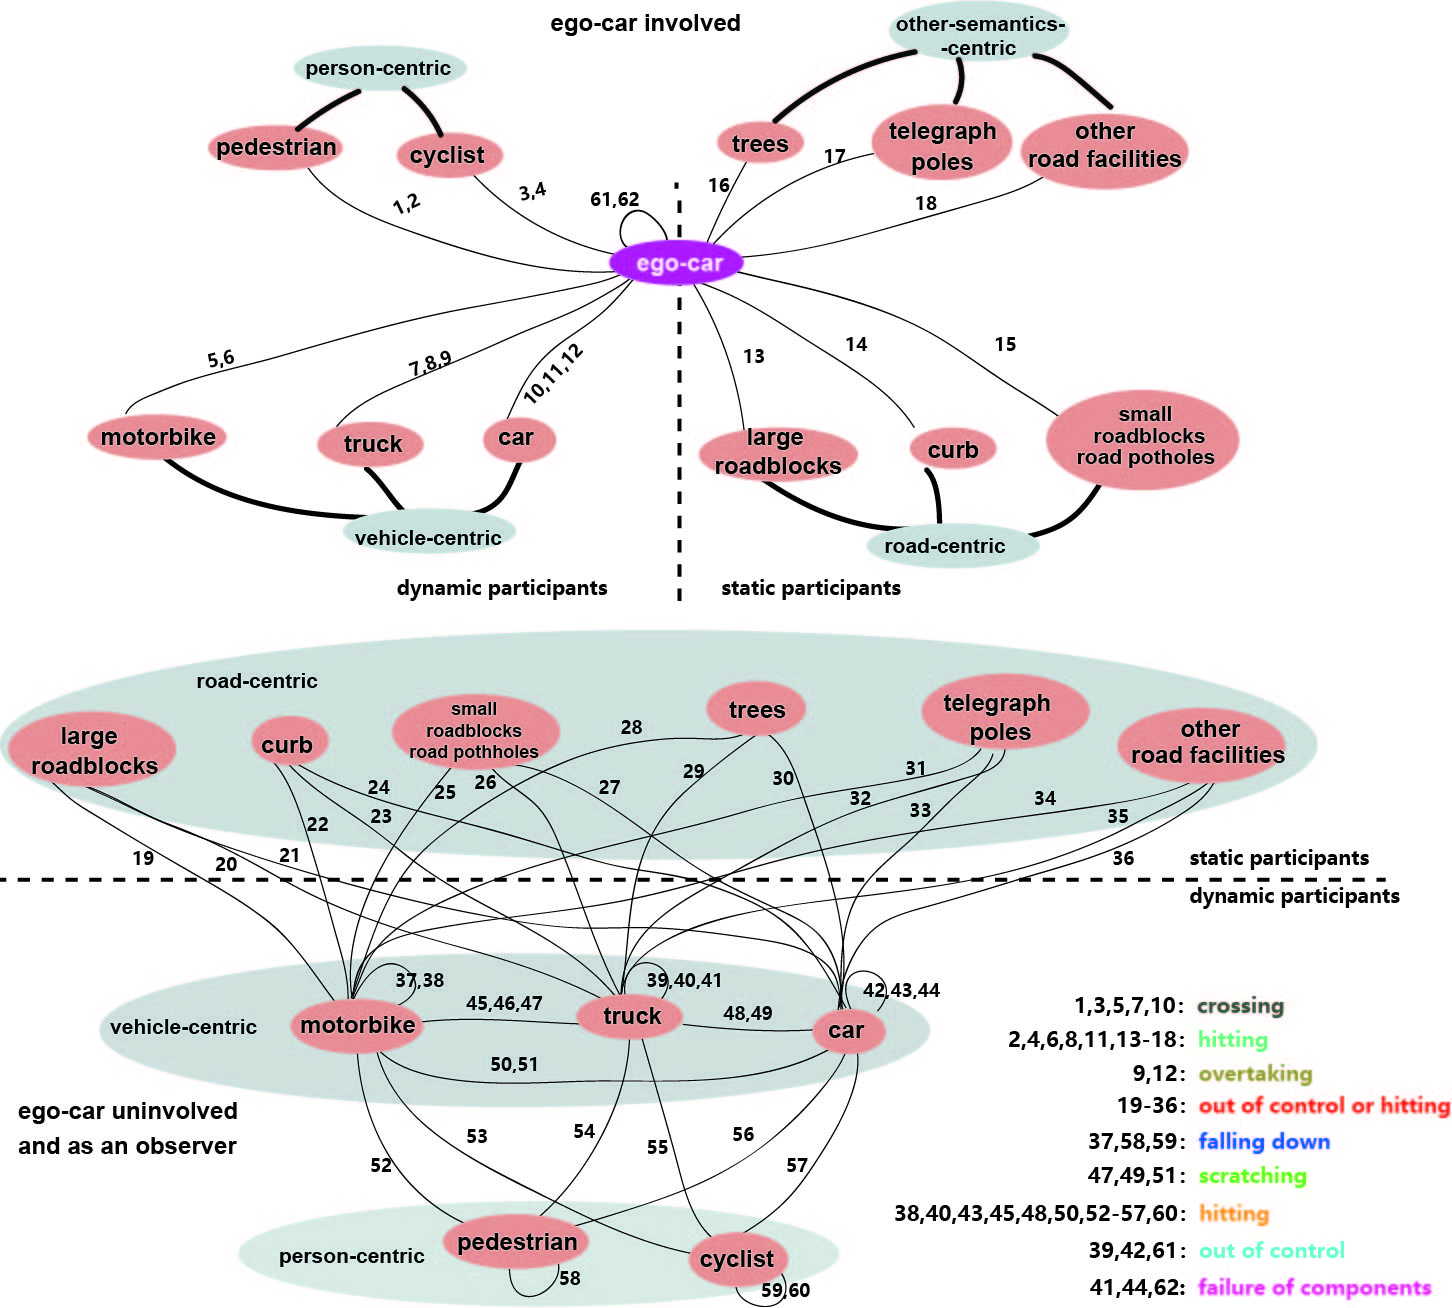
\includegraphics[width=0.85\linewidth]{figures/accident_classification.jpg}
    \caption{Kategorije incidenata u skupu DADA-2000.\supercite{dada2000github}}
    \label{fig:dada_categories}
\end{figure}

\subsection{Anotacije i oznake}
Anotacije u DADA-2000 zapisu nalaze se u CSV tablici gdje svaki red predstavlja jedan video-zapis i njegov opis kroz unaprijed definirane stupce. Zaglavlje eksplicitno definira kodirane kontekstne oznake: \textit{weather (sunny, rainy, snowy, foggy) 1--4}, \textit{light (day, night) 1--2}, \textit{scenes (highway, tunnel, mountain, urban, rural) 1--5} i \textit{linear (arterials, curve, intersection, T-junction, ramp) 1--5}. Uz to su navedeni \textit{type}, binarna oznaka \textit{whether an accident occurred (1/0)}, okvirni markeri \textit{abnormal start frame}, \textit{accident frame}, \textit{abnormal end frame}, \textit{total frames} te intervalni stupci \textit{[0,tai]}, \textit{[tai,tco]}, \textit{[tai,tae]}, \textit{[tco,tae]} i \textit{[tae,end]}. Na kraju svaki zapis sadrži i tekstualna polja \textit{texts}, \textit{causes} i \textit{measures}, koja opisuju događaj, uzrok i preporučenu mjeru.

\subsection{Uvjeti snimanja i scenariji}
Uvjeti snimanja u DADA-2000 označeni su atributima \textit{weather} (sunčano, kiša, snijeg, magla) i \textit{light} (dan/noć). Kontekst vožnje opisan je stupcima \textit{scenes} (autocesta, tunel, planinsko, urbano i ruralno okruženje) te \textit{linear} (arterija, zavoj, raskrižje, T-raskrižje, rampa). Svaki zapis dodatno sadrži tip incidenta (\textit{type}) i oznaku je li nesreća nastupila (\textit{1/0}), pa je moguće analizirati scenarije kroz različite kombinacije uvjeta.

\section{Organizacija lokalnih podataka}
Podtci DADA-2000 skupa organizirani su unutar lokalnog projekta radi jednostavnijeg učitavanja, pretraživanja i obrade. Naglasak je na praktičnom tijeku rada: od izgradnje lokalnog indeksa, preko učitavanja i pregleda videozapisa, do odabira podskupova za buduće testove.

\subsection{Izgradnja lokalnog indeksa}
Lokalni indekser uveden je kako bi se rad sa skupom DADA-2000 ubrzao i standardizirao prije same obrade videa. Umjesto da sustav pri svakom pokretanju ponovno prolazi kroz cijelu strukturu direktorija i ručno usklađuje zapise iz CSV anotacija, indekser jednom prolazi kroz dataset, prikuplja metapodatke o zapisima i sprema ih u SQLite\supercite{sqlite} bazu s dvije povezane tablice (zapisi i anotacije). Ključ povezivanja je kombinacija kategorije i video ID-a, pa se odmah može označiti je li zapis ispravno uparen, nedostaje li anotacija ili je ključ dvosmislen. Takav pristup omogućuje brže dohvaćanje pojedinog videa, filtriranje po kategoriji i direktni dohvat spojenih podataka bez ponovnog parsiranja izvora. Dodatno, izgradnja indeksa radi atomski (privremena baza pa zamjena), što smanjuje rizik od djelomično zapisanih ili nekonzistentnih podataka. Bez ovog koraka pipeline bi bio sporiji, osjetljiviji na greške u mapiranju i teže ponovljiv između različitih pokretanja.

\subsection{Učitavanje i pregled videa}
Učitavanje videa u projektu kreće od lokalnog indeksa: za zadani \textit{category\_id} i \textit{video\_id} dohvaća se točan zapis i putanja do podataka, a zatim se po potrebi preusmjeri na mapu \textit{images} ako je zapis inicijalno vezan uz pomoćne mape poput \textit{fixation} ili \textit{maps}. Okviri se zatim iteriraju preko parsera koji podržava i sekvence slika i video datoteke, pri čemu se svaki okvir referencira kroz \textit{frame\_ref} i učitava tek kada je potreban. U scenarijskom pokretanju odabrani video se unaprijed predmemorira u RAM, što omogućuje stabilniji prikaz, brže pomicanje po frameovima i manje oscilacije zbog ponovljenih pristupa disku. Za pregled i provjeru zapisa koristi se poseban player koji nad okvirom prikazuje i oznaku stanja (\textit{normal}, \textit{abnormal}, \textit{accident\_frame}) na temelju anotiranih granica događaja.
% !TeX root = ../main.tex
\chapter{Metodologija}
U ovom poglavlju opisana je metodologija kojom je izgrađen ADAS sustav, s naglaskom na dizajnerske odluke, tok obrade i razlog odabira konkretnih pristupa u svakoj fazi. Za razliku od teorijskog dijela koji opisuje koncepte i matematičke osnove, ovdje je fokus na tome kako su ti koncepti primijenjeni i kako međusobno djeluju u cjelovitom sustavu. Poseban naglasak stavljen je na kontekstno svjestan pristup koji prilagođava parametre detekcije i logiku odlučivanja prema procjeni kvalitete scene u trenutku izvođenja. Takav pristup nije samo tehnička odluka nego i odgovor na stvarna ograničenja sustava koji se oslanja isključivo na jednu prednju kameru bez podataka o brzini, dubini ili vanjskim senzorima.

\section{Metodološki okvir i tok obrade}
Sustav je izgrađen kao modularan deterministički \textit{pipeline} u kojemu svaki korak obrade prima jasno definirani ulaz i producira jasno definirani izlaz. Takav pristup olakšava zamjenu pojedinih komponenti, testiranje u izolaciji i razumijevanje uzroka svake odluke sustava. Konceptualni redoslijed faza unutar jednog okvira je sljedeći: dohvat slike iz predmemorije, kontekstna analiza scene, detekcija prometnih traka, detekcija i praćenje prepreka, procjena rizika sudara, logika odlučivanja te prikaz rezultata kroz korisničko sučelje. Svaki od modula prima izlaz prethodnih faza i kontekstno stanje, čime se parametri prilagođavaju sceni koja se trenutno obrađuje.

Jedan od ključnih dizajnerskih izbora je odvajanje kontekstne analize od ostatka \textit{pipeline-a} u zasebnu pozadinsku dretvu. Kontekstna analiza, koja procjenjuje vidljivost, stanje površine i dostupnost traka, računski je skuplja od ostalih modula i nije nužno potrebna za svaki okvir. Zbog toga je implementirana klasa \textit{ContextService} koja pokreće vlastitu \textit{daemon} dretvu i asinkrono obrađuje dolazne okvire. Glavna petlja šalje okvire pozadinskoj dretvi putem neblokirajućeg poziva \texttt{push\_frame()}, a zatim odmah čita posljednje dostupno kontekstno stanje putem \texttt{get\_state()}. Ako analiza još nije završena, koristi se prethodno stanje, čime se izbjegava čekanje i osigurava konzistentna brzina obrade. Kontekst se ne računa za svaki okvir, nego svakih \textit{N} okvira (zadana vrijednost je svakih 5), što dodatno smanjuje opterećenje procesora. Ako nova analiza stigne dok prethodna još nije preuzeta, stari neobrađeni okvir se odbacuje i zadržava samo najnoviji.

\begin{figure}[H]
    \centering
    \includegraphics[width=0.95\linewidth]{DijagramDretvi.png}
    \caption{Dretveni model izvršavanja sustava: glavna petlja obrade okvira i pozadinska kontekstna analiza}
    \label{fig:dada_categories}
\end{figure}

Kako bi se izbjeglo čitanje s diska unutar vremenske petlje, svi okviri videa učitavaju se u RAM memoriju u fazi inicijalizacije, prije nego što petlja krene. Rezultat je rječnik \textit{frame cache} koji preslikava indeks okvira u matricu slike. Time se osigurava predvidivo i nisko vrijeme dohvata u svakoj iteraciji petlje, neovisno o brzini pohrane ili dekodiranja. Slijed inicijalizacije prati sljedeći redoslijed: dohvat zapisa iz SQLite indeksa, izgradnja iteratora okvira, punjenje predmemorije, inicijalizacija svih modula i pokretanje kontekstnog servisa, a tek onda ulazak u glavnu petlju obrade.

Svaki modul (\texttt{LaneProcessor}, \texttt{Detector}, \texttt{SimpleTracker}, \texttt{RiskEstimator} i \texttt{decide()}) inicijalizira se jednom i zadržava interno stanje kroz sve okvire. To znači da je svaki od njih statefull u smislu da pamti prethodne rezultate i koristi ih za stabilizaciju, ovakvim pristupom . 

Osim obrade, sustav bilježi značajne događaje (pokretanje videa, promjene moda, upozorenja, kočenja) u JSONL log datoteku za kasniju analizu. Zvučno upozorenje aktivira se s minimalnim razmakom od 30~okvira između uzastopnih alertova kako bi se izbjeglo prečesto oglašavanje u nestabilnim scenama.

\section{Kontekstno usmjeravanje sustava}
Procjena vidljivosti scene temelji se na četiri metrike koje se računaju isključivo iz gornjeg dijela slike (zadano: 65\% visine okvira) kako bi se isključio donji dio snimke s asfaltom i haubom vozila. Te metrike su normalizirani kontrast, varijanca Laplacijevog gradijenta kao mjera zamućenosti, gustoća rubova i udio previše exponiranih piksela kao mjera odsjaja. Kombiniraju se u ukupnu ocjenu pouzdanosti vidljivosti kao težinska suma s vrijednostima $w_{\text{kontrast}} = 0{,}20$, $w_{\text{zamućenost}} = 0{,}30$, $w_{\text{rubovi}} = 0{,}38$ i $w_{\text{odsjaj}} = 0{,}12$, pri čemu su rasponi normalizacije kalibrirani prema stvarnim karakteristikama DADA-2000 snimki dash kamere, a ne prema vrijednostima tipičnim za kamere visoke rezolucije. Prag koji dijeli dobru od degradirane vidljivosti postavljen je na $t_{\text{vis}} = 0{,}5$. Noćna detekcija implementirana je dvojnim putem: primarni put provjerava nalazi li se 25. percentil svjetline ispod praga 55, što ukazuje na to da više od 75\% scene pripada tamnim tonovima, dok je sekundarni put rezervna kombinacija 5. percentila i srednje vrijednosti. U slučaju detekcije atmosferskog zamućenja (magle, kiše ili sl.) primjenjuje se metoda \textit{Dark Channel Prior} kojom se razlikuje maglena scena od scene s direktnim solarnim odsjajem, jer ta dva slučaja daju sličan globalni \textit{glare score} ali bitno različit lokalni signal u cestovnom dijelu slike.

Pouzdanost traka računa se heurističkom detekcijom u modulu \texttt{lane\_heuristic} unutar regije od interesa. Sirovi rezultat detekcije zaglađuje se eksponencijalnim pomičnim prosjekom s faktorom $\alpha = 0{,}3$ koji daje veću težinu novijim mjerenjima uz postupno zaboravljanje starih. Prag za minimalnu prisutnost traka postavljen je na $t_{\text{lane\_low}} = 0{,}10$, što je namjerno niža vrijednost od praga pune pouzdanosti ($t_{\text{lane}} = 0{,}6$), jer u urbanim scenama s isprekidanim oznakama, odbijanjima svjetlosnih zraka i raskrižjima čak i isprekidana Houghova transformacija nosi korisnu informaciju o geometriji ceste.

Procjena stanja podloge provodi se iz donjeg dijela regije od interesa uz isključenje donjih 20\% okvira koji odgovaraju haubu vozila. Algoritam kombinira mjeru hrapavosti teksture i uniformnosti boje kako bi klasificirao podlogu u četiri kategorije: suha asfaltna, mokra asfaltna, šljunčana ili nepoznata. Svaka kategorija nosi korekcijski faktor zaustavljanja koji iznosi $1{,}0$ za suhu asfaltnu, $1{,}4$ za mokru, $2{,}0$ za šljunčanu i $1{,}2$ za nepoznatu podlogu. Na temelju kombinacije ocjene vidljivosti i pouzdanosti traka router primjenjuje matricu odluke s četiri ishoda: ako su prisutne i trake i dobra vidljivost aktivan je \textit{normal\_marked} mod, trake bez dobre vidljivosti daju \textit{degraded\_marked}, dobra vidljivost bez traka daje \textit{unmarked\_good\_vis}, a bez oboje \textit{unmarked\_degraded}. Svaka promjena moda potvrđuje se tek nakon $k = 5$ uzastopnih okvira s istim kandidatnim modom.



\section{Detekcija traka, prepreka i praćenje objekata}

Detekcija prometnih traka provodi se unutar klase \texttt{LaneProcessor} koja prima aktivno kontekstno stanje i prema njemu prilagođava strategiju preprocesiranja. U standardnim uvjetima slika prolazi pretvorbu u sivine, Gaussovo zaglađivanje i Cannyjevu detekciju rubova, a iz rezultirajuće rubne mape Houghovom transformacijom unutar zadanog ROI-a izdvajaju se kandidati linija. Geometrija trake modelira se polinomom drugog stupnja $x(y) = ay^2 + by + c$, a koeficijenti se procjenjuju metodom najmanjih kvadrata iz skupa detektiranih točaka. Koeficijenti polinoma ne resetiraju se između okvira nego se temporalno prigušuju prema prethodno prihvaćenom stanju, čime se sprječava nagli skok geometrije trake između uzastopnih okvira čak i kada detekcija u jednom okviru nije potpuna. U degradiranom modu, umjesto standardnog Gaussovog zamućenja, primjenjuje se CLAHE ekvilizacija histograma (napredno lokalno pojačavanje kontrasta) i bilateralni filtar (pametni filter koji briše "snijeg" i šum sa slike, ali ne muti oštre rubove) koji bolje čuvaju rubove uz agresivniju redukciju šuma u uvjetima slabog kontrasta ili mokre ceste.

Detekcija prepreka radi tako da algoritam (MOG2) neprestano uči kako izgleda statična pozadina ceste. Sve što se na slici pojavi, a statistički odskače od tog modela pozadine, sustav automatski prepoznaje kao objekt u pokretu (prepreku). Analizira se samo središnji dio okvira (ROI) kako bi se isključili nebo i vozilo, dok se objekti manji od 400~px² ignoriraju kao šum. Osjetljivost sustava (MOG2 prag od 50{,}0) automatski se povećava u lošim uvjetima kako bi se vozila prepoznala i pri slabom kontrastu. Udaljenost se računa pomoću osnovnog modela kamere, uz pretpostavljenu visinu vozila $h_{\text{obj}} = 1{,}5$~m i žarišnu duljinu $f = 700$~px, prema formuli:
\begin{equation}
    d = \frac{f \cdot h_{\text{obj}}}{h_{\text{px}}}
\end{equation}
gdje je $h_{\text{px}}$ izmjerena visina omeđujućeg pravokutnika u pikselima. Ova procjena nije apsolutno točna, ali daje dovoljno konzistentne informacije za kasniju procjenu rizika u uvjetima bez dubinskog senzora.

Modul \texttt{SimpleTracker} prati objekte kroz okvire računajući njihovo preklapanje (\textit{Intersection over Union} - IoU). Ako se nova detekcija dovoljno preklapa s postojećom, njezina se pozicija ažurira; u suprotnom, sustav je registrira kao novi objekt. Takvo kontinuirano praćenje neophodno je za kasnije računanje relativne brzine.


\section{Procjena rizika i logika odlučivanja}

Za svaku praćenu prepreku modul \texttt{RiskEstimator} gradi procjenu rizika iz tri komponente: blizine objekta normalizirane prema maksimalnoj relevantnoj udaljenosti od 40~m, TTC vrijednosti i bočnog položaja objekta u odnosu na ego-traku (imaginarna traka ispred vozila prema kojoj se isto stalno kreće). Relativna brzina izvodi se iz promjene procijenjene udaljenosti između uzastopnih okvira, a TTC kao omjer trenutne udaljenosti i te relativne brzine. Svaka komponenta normalizira se na interval $[0, 1]$ i kombinira u ukupni \textit{risk score} težinskom sumom, pri čemu bočni položaj nosi smanjenu težinu za objekte koji se nalaze izvan ego-trake. Objekti procijenjeni dalje od 40~m zanemaruju se u trenutnoj iteraciji.

Modul \texttt{decide()} prevodi \textit{risk score} i TTC u jednu od tri akcije: NONE, WARN ili BRAKE. Prag za upozorenje je $t_{\text{warn}} = 0{,}35$, a prag za kočenje $t_{\text{brake}} = 0{,}65$ (ovi parametri mogu biti podložni promjenama). TTC djeluje kao neovisna komponenta hitnosti: vrijednost ispod 3{,}0~s aktivira barem WARN, a ispod 1{,}5~s aktivira BRAKE neovisno o iznosu \textit{risk score}-a. Akcija BRAKE aktivira se isključivo za objekte koji su klasificirani kao unutar ego-trake, dok WARN može biti aktiviran i za objekte izvan trake ako je \textit{risk score} dovoljno visok.

Stanje podloge iz kontekstnog modula izravno utječe na pragove odlučivanja. Na temelju \textit{braking\_multiplier} $m_b$ računa se korekcija praga
\begin{equation}
    p = 0{,}08 \cdot \max(0,\; m_b - 1{,}0)
\end{equation}
kojom se efektivni pragovi snižavaju: na mokroj podlozi ($m_b = 1{,}4$) sniženje iznosi $p = 0{,}032$, a na šljunčanoj ($m_b = 2{,}0$) iznosi $p = 0{,}08$. Rezultat je da isti \textit{risk score} na lošijoj podlozi ranije prelazi prag za aktivaciju, što u logici odlučivanja odražava stvarno povećanu opasnost koja nastaje zbog dužeg zaustavnog puta vozila.


\section{Integracija i stabilizacija rada kroz slijed okvira}
Stabilnost sustava rješava se unutar samih modula, a ne centralno. Kontekstni router koristi histerezu ($k = 5$ okvira) kako bi spriječio "titranje" modova. \texttt{LaneProcessor} zaglađuje promjene kako bi izbjegao nagle skokove traka, \texttt{SimpleTracker} prati objekte preko IoU-a, a \texttt{RiskEstimator} računa brzinu iz razlike udaljenosti.

Moduli ne komuniciraju direktno, već svi čitaju isti \texttt{ContextState} objekt, što znatno olakšava odvojeno testiranje. Ovisno o tom kontekstu, moduli prilagođavaju svoje parametre (MOG2 prag, CLAHE, pragovi kočenja).

Kako bi se izbjeglo neprestano pištanje na granici detekcije, zvučno upozorenje ima \textit{cooldown} od 30~sličica. Svi bitni događaji (WARN, BRAKE, promjene modova) logiraju se u JSONL datoteku radi lakšeg \textit{debuggiranja} i provjere pomoću DADA-2000 \textit{dataseta}.
% !TeX root = ../main.tex

\chapter{Implementacija}

U ovom poglavlju opisana je konkretna implementacija ADAS sustava: od alata i okruženja u kojemu je razvijen, preko organizacije modula i paketa, do načina testiranja i korisničkog sučelja. Naglasak nije samo na opisu što je izgrađeno, nego i na objašnjenju zašto su određeni alati i pristupi odabrani. Sav izvorni kod projekta javno je dostupan na repozitoriju\supercite{adasgithub}.

\section{Korištene javne biblioteke}

Projekt je napisan u Pythonu 3.12 i oslanja se na manji skup dobro poznatih biblioteka. Cilj je bio svesti vanjske ovisnosti na minimum i koristiti isključivo biblioteke koje imaju stabilan API i dobru dokumentaciju.

\textbf{OpenCV}\supercite{opencv} (\texttt{opencv-python}) je središnja biblioteka za sve operacije računalnog vida u projektu. Koristi se u gotovo svim paketima: u \texttt{lane\_detection} za pretvorbu slike u jedan \textit{grayscale} kanal, Gaussovo zaglađivanje, Canny detekciju rubova, CLAHE preprocesiranje i Houghovu transformaciju; u \texttt{obstacle\_detection} za MOG2 oduzimanje pozadine, morfološke operacije i ekstrakciju kontura; u \texttt{context} za izračun metrika slike poput varijance Laplacijevog gradijenta; te u \texttt{ui} za iscrtavanje rezultata i pokretanje prozora za pregled.

\textbf{NumPy} (\texttt{numpy}) koristi se kao osnova za sve numeričke operacije nad matricama slika. Većina izlaza OpenCV funkcija su NumPy nizovi, pa je ova biblioteka inherentno prisutna u gotovo svakom modulu koji radi s okvirima.

\textbf{scikit-image} (\texttt{scikit-image}) koristi se u modulu za procjenu stanja ceste (\texttt{context/ road\_surface.py}), gdje se primjenjuje za analizu teksture površine radi razlikovanja asfaltirane, mokre i šljunčane podloge.

\textbf{scikit-learn} (\texttt{scikit-learn}) koristi se za pomoćne statističke operacije, posebno u modulima koji trebaju normalizaciju ili jednostavne numeričke transformacije.

\textbf{Pillow} (\texttt{pillow}) koristi se za učitavanje i konverziju slika na mjestima gdje je potrebna šira podrška za formate datoteka od one koju nudi OpenCV, primjerice pri generiranju sličica (\textit{thumbnails}) u korisničkom sučelju.

\textbf{Dear PyGui} (\texttt{dearpygui}) je biblioteka za izgradnju grafičkih korisničkih sučelja temeljena na GPU renderiranju. Koristi se za implementaciju glavnog upravljačkog panela (\texttt{ui/master\_panel.py}) koji objedinjuje pregled videa, tablicu zapisa iz dataseta, konfiguraciju parametara i prikaz statusa.

Za razvoj se koriste i razvojne ovisnosti: \texttt{pytest} za pokretanje automatiziranih testova, \texttt{ruff} za statičku analizu koda (\textit{linting}), \texttt{black} za automatsko formatiranje i \texttt{pre-commit} za provjere prije svake predaje izmjena u repozitorij. Uz to je uključen i \texttt{jupyterlab} za potencijalnu interaktivnu analizu u Jupyter bilježnicama.

\section{Postavljanje radnog okruženja}

\subsection{Razvojno okruženje}

Projekt je razvijen u Visual Studio Code (\textit{VS Code}) uz ekstenziju \textit{Dev Containers} koja omogućuje pokretanje razvojnog okruženja unutar Docker kontejnera. Prednost ovakvog pristupa je u tome što svaki razvojnik dobiva identično okruženje bez ručnog postavljanja Python verzija, biblioteka ili LaTeX paketa. Repozitorij se klonira i otvara u VS Code-u, a zatim se jednom naredbom (\textit{Reopen in Container}) pokreće izgradnja kontejnera u kojemu se odvija sav razvoj, pokretanje koda i kompajliranje dokumentacije.

\subsection{Struktura projekta}

Projekt je organiziran u nekoliko direktorija s jasno odvojenim ulogama:
\begin{itemize}
    \item \texttt{src/} -- izvorni kod Python paketa (jedino mjesto gdje živi logika sustava)
    \item \texttt{tests/} -- automatizirani testovi, zrcalna struktura kao \texttt{src/}
    \item \texttt{scripts/} -- pomoćne skripte za pokretanje scenarija, debug vizualizaciju i upravljanje datasetom
    \item \texttt{data/} -- sirovi i obrađeni podaci (DADA-2000 skup i SQLite indeks)
    \item \texttt{docs/} -- LaTeX izvorni kod ovog rada
    \item \texttt{dep/} -- unaprijed preuzete binarne ovisnosti (PulseAudio za Windows)
\end{itemize}

\subsection{Docker i grafičko sučelje}

Docker kontejner se gradi iz \texttt{Dockerfile}-a koji instalira Python 3.12, Poetry, sve Python ovisnosti i kompletan LaTeX distribuciju (\texttt{texlive-full}). Za grafički prikaz prozora iz kontejnera na Windows hostu potreban je X server. U projektu se koristi \textbf{VcXsrv} koji prima X11 protokol i renderira prozore na Windows desktopu. Konfiguracija je postavljena u \texttt{docker-compose.yml} koji postavlja varijable okoline \texttt{DISPLAY}, \texttt{QT\_QPA\_PLATFORM} i \texttt{QT\_X11\_NO\_MITSHM} kako bi OpenCV prozori ispravno funkcionirali.

Za zvučna upozorenja (WARN i BRAKE alertovi) Docker kontejner nema izravni pristup zvučnoj kartici hosta pa se koristi \textbf{PulseAudio} kao posredni server za audio tok. Kako korisnici ne bi morali ručno instalirati PulseAudio, binarne datoteke su uključene direktno u repozitorij unutar direktorija \texttt{dep/pulseaudio-1.1/}. Na Windows hostu se pokreće priložena skripta koja PulseAudio pokreće kao lokalni server koji kontejner može doseći putem mrežne adrese hosta.

\begin{lstlisting}[style=bashcode, caption={Pokretanje PulseAudio servera na Windows hostu}, label={lst:pulseaudio}]
scripts\start_pulseaudio.bat
\end{lstlisting}

\subsection{Upravljanje ovisnostima i Makefile}

Upravljanje Python ovisnostima riješeno je alatom \textbf{Poetry}. Sve ovisnosti i ograničenja verzija definirane su u datoteci \texttt{pyproject.toml}, a točne verzije zabilježene su u \texttt{poetry.lock} datoteci kako bi svaki \textit{build} bio jasno reproducibilan. Razvojne ovisnosti (\texttt{pytest}, \texttt{ruff}, \texttt{black}, \texttt{pre-commit}) odvojene su u zasebnu grupu kako ne bi bile instalirane u produkcijskim scenarijima.

Za najčešće naredbe postoji \texttt{Makefile} koji skraćuje dugačke pozive u terminalu. Na primjer:

\begin{lstlisting}[style=bashcode, caption={Najčešće Makefile naredbe}, label={lst:makefile}]
make install         # instalira ovisnosti putem Poetry
make test            # pokreće sve testove
make lint            # ruff statička provjera koda
make format          # black automatsko formatiranje
make build           # docker compose build
make up              # docker compose up
\end{lstlisting}

\subsection{Verzioniranje i CI/CD}

Kod je verzioniran sustavom \textbf{Git}, a repozitorij je smješten na GitHubu.\supercite{adasgithub} Svaka predaja izmjena na glavnu granu (\texttt{main}) ili svaki zahtjev za spajanjem (\textit{pull request}) pokreće automatiziranu provjeru putem \textbf{GitHub Actions}. Definirani CI/CD \textit{pipeline} radi sljedeće korake: postavlja Python 3.12, instalira Poetry i ovisnosti, pokreće \texttt{ruff} statičku provjeru koda te naposljetku izvršava cijeli skup automatiziranih testova putem \texttt{pytest}. Na taj način svaka promjena u kodu automatski prolazi kroz provjeru ispravnosti prije nego što bude prihvaćena u glavnu granu.

\begin{figure}[H]
    \centering
    \includegraphics[width=0.85\linewidth]{ci_github.png}
    \caption{Prikaz GitHub Actions CI/CD \textit{pipeline-a} s koracima provjere koda i testiranja.}
    \label{fig:ci_github}
\end{figure}

\section{Arhitektura sustava i organizacija modula}

\subsection{Organizacijski pojmovi}

U Pythonu je \textbf{paket} direktorij koji sadrži datoteku \texttt{\_\_init\_\_.py} i može obuhvaćati više \textbf{modula}. Modul je pojedinačna \texttt{.py} datoteka s funkcijama, klasama i konstantama. U ovom projektu sav izvorni kod nalazi se unutar paketa \texttt{adas} koji je smješten u direktoriju \texttt{src/adas/}. Unutar njega postoje podpaketi koji odgovaraju pojedinim funkcionalnim cjelinama sustava. Varijabla okoline \texttt{PYTHONPATH=/app/src} osigurava da Python interpreter može pronaći paket \texttt{adas} bez instaliranja u sistemski \textit{site-packages}.

\begin{figure}[H]
    \centering
    \includegraphics[width=0.30\linewidth]{pkg_struktura.png}
    \caption{Struktura paketa projekta unutar direktorija \texttt{src/adas/}.}
    \label{fig:pkg_struktura}
\end{figure}

\subsection{Paket \texttt{context}}

Paket \texttt{context} odgovoran je za procjenu kvalitete scene i usmjeravanje sustava prema odgovarajućem načinu rada. Sadrži sljedeće module:

\begin{itemize}
    \item \texttt{scene\_metrics.py} -- računa metrike slike (svjetlina, zamućenost, gustoća rubova, odsjaj) i iz njih gradi ocjenu vidljivosti; ujedno implementira \textit{Dark Channel Prior} za razlikovanje magle od odsjaja
    \item \texttt{lane\_heuristic.py} -- heuristička detekcija prisutnosti traka unutar definirane regije od interesa
    \item \texttt{lane\_state.py} -- kombinira sirovi signal detekcije s konfigurabilnim pragovima u formalni \texttt{LaneState} objekt
    \item \texttt{road\_surface.py} -- procjena stanja podloge (suha, mokra, šljunčana, nepoznato) iz donjeg dijela slike; određuje \textit{braking\_multiplier} koji se propagira u modul procjene rizika
    \item \texttt{router.py} -- kombinira procjene vidljivosti i stanja traka u jedan od četiri radna moda sustava uz mehanizam histereze
    \item \texttt{service.py} -- \texttt{ContextService} klasa koja pokreće kontekstnu analizu u pozadinskoj dretvi i nudi neblokirajući pristup posljednjem rezultatu
    \item \texttt{defaults.py} -- sve numeričke konstante i pragovi u jednoj konfiguracijskoj klasi (\texttt{ContextConfig}) koja se može nadjačati putem runtime JSON datoteke
    \item \texttt{types.py} -- definicija svih tipova podataka paketa: ContextState, Mode, VisibilityEstimate i slično
\end{itemize}

Javno sučelje paketa svodi se na jednu glavnu funkciju \texttt{route(frame, ...)} i klasu \texttt{ContextService} za asinkronu uporabu u petlji obrade. Isječak~\ref{lst:context_route} prikazuje tipičan poziv unutar glavne petlje:

\begin{lstlisting}[style=pycode, caption={Korištenje \texttt{ContextService} u glavnoj petlji obrade}, label={lst:context_route}]
ctx_service = ContextService(config=DEFAULT_CONFIG, context_interval=5)
ctx_service.start()

# unutar glavne petlje:
ctx_service.push_frame(frame, frame_idx, timestamp_s=ts, fps=30.0)
ctx_state = ctx_service.get_state()  # nikad ne blokira
\end{lstlisting}

\subsection{Paket \texttt{lane\_detection}}

Paket \texttt{lane\_detection} implementira detekciju prometnih traka iz pojedinačnih okvira uz privremenu stabilizaciju između okvira. Sadrži sljedeće module:

\begin{itemize}
    \item \texttt{processing.py} -- središnji modul koji implementira \texttt{LaneProcessor} klasu s unutarnjim stanjem i \texttt{process\_frame()} funkcijskim sučeljem; uključuje standardni put pretprocesiranja (spomenuti CLAHE + bilateralni filtar), Houghovu detekciju kandidata i polinomsko \textit{namještanje} s prigušivanjem koeficijenata prema prethodnom stanju
    \item \texttt{visualization.py} -- pomoćne funkcije \texttt{draw\_lanes()} i \texttt{draw\_edges()} za iscrtavanje rezultata detekcije na okvir; ovdje se crta i ego traka
    \item \texttt{metrics.py} -- \texttt{evaluate\_detection()} i \texttt{evaluate\_batch()} za vrjednovanje ispravnosti detekcije traka
    \item \texttt{hough.py} -- geometrijska detekcija traka temeljena na Houghovoj transformaciji s višerazinskim skupljanjem segmenata, RANSAC-robusnim polinomskim namještanjem i Kalmanovim filterom za vremensku stabilizaciju; integriran u \texttt{processing.py} kao primarni motor detekcije
\end{itemize}

\begin{lstlisting}[style=pycode, caption={Poziv detekcije traka unutar glavne petlje}, label={lst:lane_proc}]
lane_processor = LaneProcessor()

# unutar glavne petlje:
lane_output = lane_processor.update(frame, ctx_state)
\end{lstlisting}

\subsection{Paket \texttt{obstacle\_detection}}

Paket \texttt{obstacle\_detection} implementira detekciju i praćenje objekata u prometnoj sceni. Sadrži sljedeće module:

\begin{itemize}
    \item \texttt{detector.py} -- \texttt{Detector} klasa koja koristi MOG2 algoritam oduzimanja pozadine za izdvajanje prednjeg plana, morfološke operacije za čišćenje šuma i filtriranje kontura prema veličini, obliku i poziciji unutar ROI-a; procjena udaljenosti temelji se na heuristici s pretpostavljenom visinom objekta i kalibriranom žarišnom duljinom; parametri se dinamički prilagođavaju prema kontekstnom stanju
    \item \texttt{tracking.py} -- \texttt{SimpleTracker} koji dodjeljuje stabilne identifikatore objektima kroz uzastopne okvire temeljem IoU mjere preklapanja omeđujućih pravokutnika
    \item \texttt{types.py} -- \texttt{DetectedObject} dataklasa koja opisuje jedan detektirani objekt: identifikator, omeđujući pravokutnik, procijenjenu udaljenost, lateralni položaj i zastavicu je li unutar ego-trake
    \item \texttt{metrics.py} -- \texttt{evaluate\_detections()} za vrjednovanje detekcija nasuprot referentnih anotacija
\end{itemize}

\begin{lstlisting}[style=pycode, caption={Detekcija i praćenje prepreka}, label={lst:obstacle}]
detector = Detector()
tracker = SimpleTracker()

# unutar glavne petlje:
raw_detections = detector.detect(frame, lane_output=lane_output,
                                 context_state=ctx_state)
tracked = tracker.update(raw_detections)
\end{lstlisting}

\subsection{Paket \texttt{collision\_risk}}

Paket \texttt{collision\_risk} pretvara listu praćenih objekata u konkretnu preporuku za akciju. Sadrži sljedeće module:

\begin{itemize}
    \item \texttt{estimator.py} -- \texttt{RiskEstimator} koji za svaki praćeni objekt izračunava TTC, blizinu i lateralni položaj te ih kombinira u numerički \textit{risk score}; relativna brzina izvodi se iz promjene procijenjene udaljenosti između okvira uz kratki klizeći buffer
    \item \texttt{decision.py} -- \texttt{decide()} funkcija koja uspoređuje \textit{risk score} i TTC s konfigurabilnim pragovima te vraća jednu od tri akcije (\texttt{NONE}, \texttt{WARN}, \texttt{BRAKE}) uz intenzitet; uzima u obzir i \textit{braking\_multiplier} iz kontekstnog stanja za prilagodbu pragova
    \item \texttt{types.py} -- \texttt{RiskResult} i \texttt{SystemAction} tipovi
    \item \texttt{metrics.py} -- \texttt{evaluate\_action()} i \texttt{aggregate\_evaluation()} za vrjednovanje akcija sustava nasuprot anotiranih oznaka nesreća iz DADA-2000
\end{itemize}

\begin{lstlisting}[style=pycode, caption={Procjena rizika i donošenje odluke}, label={lst:risk}]
risk_estimator = RiskEstimator()

# unutar glavne petlje:
risks = risk_estimator.estimate_risk(
    tracked, lane_output=lane_output,
    context_state=ctx_state, frame_idx=frame_idx
)
action, intensity = decide(risks, context_state=ctx_state)
\end{lstlisting}

\subsection{Paket \texttt{dataset}}

Paket \texttt{dataset} sadrži sve što je potrebno za rad s DADA-2000 skupom podataka. Sadrži sljedeće module:

\begin{itemize}
    \item \texttt{parser.py} -- parsiranje stabla direktorija, izgradnja iteratora okvira i dohvaćanje pojedinog okvira prema referenci; podržava sekvence slika i video datoteke
    \item \texttt{indexer.py} -- izgradnja SQLite indeksa s tablicama \texttt{records} i \texttt{annotations} iz CSV anotacijske datoteke i direktorijske strukture; pisanje se odvija atomski kroz privremenu datoteku
    \item \texttt{lotvs\_reader.py} -- čitač podataka specifičan za LOTVS/DADA format, uglavnom korišten od strane parsera
    \item \texttt{annotation.py} -- pomoćne funkcije za dohvat i interpretaciju anotacijskih podataka pojedinog video zapisa (oznake okvira, intervali, kontekstni atributi)
    \item \texttt{sampler.py} -- \texttt{random\_sample()} i \texttt{stratified\_sample()} funkcije za odabir uzoraka iz indeksa, s opcionalnim \textit{seed-om} pseudonasumičnog odabira
    \item \texttt{loader\_wrappers.py} -- omotači koji kombiniraju dohvat iz indeksa s učitavanjem okvira u jednostavno iterabilno sučelje
    \item \texttt{utils\_io.py} -- pomoćne I/O funkcije za atomsko zapisivanje datoteka i provjeru putanja
\end{itemize}

\subsection{Paket \texttt{scenario}}

Paket \texttt{scenario} orkestrira cijeli pipeline za jednu snimku. Sadrži sljedeće module:

\begin{itemize}
    \item \texttt{runner.py} -- \texttt{run\_scenario()} funkcija koja inicijalizira sve module, puni RAM predmemoriju okvira, pokreće kontekstni servis u pozadinskoj dretvi i izvršava glavnu petlju obrade; podržava normalni i \textit{streaming} mod (pisanje sličica i JSON statusa na disk za live prikaz u UI-u)
    \item \texttt{types.py} -- \texttt{ScenarioConfig} nepromjenjiva konfiguracija scenarija i \texttt{FrameResult} koji opisuje izlaz obrade jednog okvira
    \item \texttt{events.py} -- \texttt{ScenarioEvent} i \texttt{log\_event()} za bilježenje značajnih događaja u JSONL datoteku
\end{itemize}

\subsection{Paket \texttt{ui}}

Paket \texttt{ui} odgovoran je za sve što je vidljivo korisniku. Sadrži sljedeće module:

\begin{itemize}
    \item \texttt{master\_panel.py} -- glavni upravljački panel implementiran u Dear PyGui; objedinjuje tablicu zapisa iz dataseta, kartice za izgradnju indeksa, pokretanje scenarija, konfiguraciju parametara i live pregled videa
    \item \texttt{backend\_cv2.py} -- \texttt{Cv2Player} koji koristi OpenCV \texttt{imshow} za interaktivni pregled, podržava tipkovničke naredbe za reprodukciju
    \item \texttt{backend\_dpg.py} -- \texttt{DpgPlayer} koji koristi Dear PyGui za isti pregled unutar GPU-renderiranog prozora
    \item \texttt{overlays.py} -- \texttt{draw\_lanes()}, \texttt{draw\_obstacles()} i \texttt{draw\_risk()} za iscrtavanje rezultata detekcije i procjene rizika izravno na okvir
    \item \texttt{dashboard.py} -- \texttt{draw\_stats\_panel()} i \texttt{draw\_stats\_overlay()} za prikaz numeričkih metrika u uglu slike
    \item \texttt{audio.py} -- \texttt{play\_warning\_beep()} i \texttt{play\_brake\_beep()} za zvučna upozorenja; koristi PulseAudio kada je dostupan
    \item \texttt{player.py} -- generičke \texttt{create\_player()} i \texttt{run\_player\_loop()} funkcije koje apstrahiraju odabir između cv2 i dpg backenda
    \item \texttt{types.py} -- \texttt{UIState} i \texttt{UICommand} tipovi za komunikaciju između loopa obrade i UI-a
\end{itemize}

\subsection{Paket \texttt{utils}}

Paket \texttt{utils} sadrži male \textit{stateless} pomoćne funkcije. Modul \texttt{runtime\_overrides.py} implementira mehanizam kojim se numerički parametri konfiguracije mogu nadjačati u trenutku izvođenja bez mijenjanja izvornog koda: čita JSON datoteku \path{data/processed/runtime_overrides.json} i primjenjuje pronađene vrijednosti na zadani konfiguracijski dataclass. Ovaj mehanizam koriste svi konfiguracijski objekti u sustavu (\texttt{ContextConfig}, \texttt{DetectorConfig}, \texttt{EstimatorConfig}, \texttt{DecisionConfig}) pa je moguće podešavati parametre bez ponovnog pokretanja kontejnera. Isječak~\ref{lst:overrides} prikazuje strukturu te JSON datoteke.

\begin{lstlisting}[style=bashcode, caption={Primjer runtime\_overrides.json datoteke s nadjačanim parametrima}, label={lst:overrides}]
{
  "context": { "context_interval": "30" },
  "decision": { "brake_score_threshold": 0.65 },
  "obstacle": { "min_area": 400.0, "mog2_var_threshold": 50.0 },
  "lane":     { "hough_threshold": 35, "roi_top": 0.5 }
}
\end{lstlisting}

\section{Testiranje}

\subsection{Organizacija testova}

Testovi su smješteni u direktorij \texttt{tests/} koji zrcali strukturu \texttt{src/adas/}: za svaki paket postoji odgovarajući poddirektorij s test modulima. Svi testovi koriste \textbf{pytest} okvir. Pokretanje svih testova svodi se na jednu naredbu:

\begin{lstlisting}[style=bashcode, caption={Pokretanje testova}, label={lst:pytest}]
poetry run pytest tests/
# ili kraće:
make test
\end{lstlisting}

\subsection{Testiranje bez stvarnog dataseta}

Budući da DADA-2000 dataset nije dio repozitorija (velik je i preuzima se zasebno), testovi su dizajnirani tako da ne ovise o stvarnim video datotekama. Umjesto toga, za testove koji zahtijevaju slike koriste se sintetički okviri generirani NumPy-em. Primjerice, u direktoriju \texttt{tests/context/} postoji \texttt{conftest.py} koji definira \textit{pytest fixture-e}: crni okvir za simulaciju noći, bijeli okvir za simulaciju odsjaja, sivi okvir za uniformnu scenu, gradijentni okvir za umjerenu vidljivost i nasumično-šumni okvir za degradirane uvjete. Na taj se način svaki modul može testirati u izolaciji, bez ovisnosti o vanjskim podacima.

Za testove koji trebaju SQLite indeks (primjerice \texttt{test\_indexer.py} ili \texttt{test\_sampler.py}), indeks se gradi u privremenoj memorijskoj bazi (\texttt{:memory:}) ili u privremenom direktoriju koji pytest automatski uklanja nakon testa.

\subsection{Testiranje scenarija}

Test modul \texttt{tests/scenario/test\_runner.py} provjerava ponašanje \texttt{run\_scenario()} funkcije bez potrebe za stvarnim videopodacima ili grafičkim sučeljem. Koristi \texttt{unittest.mock} za zamjenu poziva koji bi zahtijevali GUI ili dataset, čime se potvrđuju konfiguracijski tipovi, logika događaja i ponašanje \texttt{ScenarioConfig} i \texttt{FrameResult} dataklasa.

\subsection{Evaluacijske metrike}

Paketi \texttt{collision\_risk}, \texttt{obstacle\_detection} i \texttt{lane\_detection} svaki imaju vlastiti modul \texttt{metrics.py} koji implementira funkcije za ocjenjivanje rezultata nasuprot referentnih anotacija. Za procjenu rizika i odlučivanja (\texttt{collision\_risk/metrics.py}) definirani su standardni pokazatelji klasifikacije: preciznost, odziv, F1-mjera i stopa lažnih alarma, računati usporedbom akcija sustava s oznakama akcidentalnih okvira iz DADA-2000 anotacija. Ovakav pristup omogućuje kvantitativnu provjeru ponašanja sustava na scenarijima za koje postoje referentne oznake.

\section{Olakšani pristup --- skripte i ulazna točka}

\subsection{Skripte u direktoriju \texttt{scripts/}}

Direktorij \texttt{scripts/} sadrži skripte koje olakšavaju najčešće zadatke pri radu s projektom. Svaka skripta je samostalna i poziva se iz korijenskog direktorija projekta (u Dockeru je to \texttt{/app}).

\textbf{\texttt{scripts/run\_scenario.py}} je glavna CLI ulazna točka za pokretanje cijelog ADAS pipeline-a nad jednim video zapisom iz dataseta. Prima argumente za odabir kategorije i video ID-a, odabir UI backenda, broj okvira, interval kontekstne analize i opcijsko isključivanje audio upozorenja. Podržava i posebni \textit{streaming} mod u kojemu svaki okvir zapisuje sličicu i JSON statusnu datoteku na disk, što koristi master panel za live prikaz bez direktnog X11 prozora.

\begin{lstlisting}[style=bashcode, caption={Pokretanje scenarija iz naredbenog retka}, label={lst:run_scenario}]
python scripts/run_scenario.py --category-id 1 --video-id 3
python scripts/run_scenario.py --category-id 2 --video-id 1 --no-audio --ui-backend cv2
\end{lstlisting}

\textbf{\texttt{scripts/debug\_lanes.py}} prikazuje samo rezultate detekcije traka (Canny rubovi, namješteni polinomi, maska trake) bez pokretanja detekcije prepreka ili procjene rizika. Koristan je pri podešavanju parametara lane detectiona.

\begin{lstlisting}[style=bashcode, caption={Debug vizualizacija detekcije traka}, label={lst:debug_lanes}]
python scripts/debug_lanes.py --category-id 1 --video-id 1 --show-edges
\end{lstlisting}

\textbf{\texttt{scripts/debug\_obstacles.py}} na sličan način prikazuje samo detekciju i praćenje prepreka. Opcionalnim argumentom \texttt{--with-lanes} moguće je dodati i vizualizaciju traka.

\begin{lstlisting}[style=bashcode, caption={Debug vizualizacija detekcije prepreka}, label={lst:debug_obs}]
python scripts/debug_obstacles.py --category-id 1 --video-id 1 --with-lanes
\end{lstlisting}

Poddirektorij \texttt{scripts/dataset/} sadrži skripte za upravljanje datasetom:
\begin{itemize}
    \item \texttt{build\_index.py} -- gradi SQLite indeks iz CSV anotacija i strukture direktorija
    \item \texttt{download\_dataset.py} -- preuzimanje DADA-2000 dataset datoteka (potencijalni problemi zbog veličine dataseta od 100+GB)
    \item \texttt{play\_index\_video.py} -- pregled pojedinog videa iz indeksa s prikazom anotacijskih oznaka okvira
    \item \texttt{export\_samples.py} -- izvoz odabranih uzoraka okvira na disk
    \item \texttt{sample\_conditions.py} -- uzorkovanje zapisa prema uvjetima (vremenski uvjeti, scenarij, dan/noć)
    \item \texttt{run\_parser.py} -- ručno pokretanje parsera za provjeru ispravnosti čitanja video izvora
    \item \texttt{upload\_dataset.py} -- pomoćna skripta za prijenos podataka (isti potencijalni problem kao i sa preuzimanjem)
\end{itemize}

Direktorij \texttt{scripts/context/} sadrži \texttt{analyze\_video.py} koji pokreće samo kontekstnu analizu nad odabranim videom i ispisuje metrike vidljivosti, stanje podloge i promjene modova okvir po okvir, bez pokretanja ostatka pipeline-a.

\subsection{Ulazna točka \texttt{main.py}}

Datoteka \texttt{main.py} u korijenu projekta je najjednostavniji način pokretanja cijelog sustava. Ona dodaje \texttt{src/} na Python putanju i poziva \texttt{run\_master\_dashboard()} koji otvara glavni Dear PyGui prozor.

\begin{lstlisting}[style=bashcode, caption={Pokretanje glavnog sučelja}, label={lst:main}]
python main.py
\end{lstlisting}

\section{Korisničko sučelje}

\subsection{Arhitektura sučelja}

Korisničko sučelje organizirano je u dva sloja. Vanjski sloj je \textbf{master panel} (\path{ui/master_panel.py}) koji se pokreće na hostu (ili unutar kontejnera s X11 prosljeđivanjem) i pruža kompletno grafičko okruženje za upravljanje projektom. Unutarnji sloj je \textbf{player prozor} koji se otvara za vrijeme reprodukcije scenarija i prikazuje obradu okvira s ucrtanim rezultatima detekcije. Ova dva sloja komuniciraju putem \textit{streaming} mehanizma: scenario runner upisuje sličice i statusne JSON datoteke na disk, a master panel ih periodički čita i prikazuje.

\subsection{Master panel}

Master panel izgrađen u Dear PyGui-u otvara se pokretanjem \texttt{main.py} i predstavlja jedinu ulaznu točku za većinu korisničkih radnji. Prozor je organiziran u nekoliko kartica:

\begin{figure}[H]
    \centering
    \includegraphics[width=0.95\linewidth]{ui_master_panel.png}
    \caption{Glavni upravljački panel (\textit{Master Dashboard}) s tablicom zapisa dataseta.}
    \label{fig:master_panel}
\end{figure}

\textbf{Kartica s tablicom zapisa} prikazuje sve zapise iz SQLite indeksa u straničenoj tablici s do 200 redaka po stranici. Svaki redak prikazuje category ID, video ID, broj okvira, putanju i anotacijske atribute (vremenske uvjete, tip scene i slično). Tablica podržava sortiranje po stupcima klikom na zaglavlje, filtriranje prema numeričkim i tekstualnim vrijednostima te odabir retka za pokretanje scenarija.

\begin{figure}[H]
    \centering
    \includegraphics[width=0.95\linewidth]{ui_tablica_filteri.png}
    \caption{Filtriranje i sortiranje tablice zapisa prema atributima anotacija.}
    \label{fig:ui_filteri}
\end{figure}

\textbf{Kartica Build Index} omogućuje izgradnju SQLite indeksa izravno iz sučelja, bez ručnog pokretanja skripte iz terminala. Prikazuje log izlaz procesa u realnom vremenu.

\textbf{Kartica Run Scenario} pruža formu za odabir parametara scenarija (category ID, video ID, FPS, interval kontekstne analize) i gumb za pokretanje. Scenarij se pokreće kao zasebni subprocess unutar kontejnera, a izlaz se struja u panel.

\begin{figure}[H]
    \centering
    \includegraphics[width=0.95\linewidth]{ui_run_scenario.png}
    \caption{Kartica za pokretanje scenarija s odabranim parametrima i prikazom loga.}
    \label{fig:ui_run_scenario}
\end{figure}

\textbf{Kartica Configurator} prikazuje live sličicu aktivnog scenarija zajedno s numeričkim statusom (trenutni mod, vidljivost, stanje traka, zadnja akcija). Ovo je koristan prikaz za praćenje ponašanja sustava u stvarnom vremenu bez potrebe za X11 prozorom.

\begin{figure}[H]
    \centering
    \includegraphics[width=0.95\linewidth]{ui_configurator.png}
    \caption{Kartica Configurator s live pregledom okvira i numeričkim statusom sustava.}
    \label{fig:ui_configurator}
\end{figure}

\textbf{Kartica Runtime Overrides} prikazuje i omogućuje uređivanje JSON datoteke s parametrima koji se nadjačavaju u izvođenju. Promjene se primjenjuju za sljedeće pokretanje scenarija bez potrebe za rekompilacijom ili ponovnim pokretanjem kontejnera.

\begin{figure}[H]
    \centering
    \includegraphics[width=0.85\linewidth]{ui_overrides.png}
    \caption{Kartica Runtime Overrides za podešavanje parametara sustava bez ponovnog pokretanja.}
    \label{fig:ui_overrides}
\end{figure}

\subsection{Player prozor}

Kada se scenarij pokreće s UI backendom \texttt{cv2} ili \texttt{dpg}, otvara se zasebni player prozor koji prikazuje video u stvarnom vremenu s ucrtanim rezultatima obrade. Na svakom okviru vidljivi su:

\begin{itemize}
    \item ucrtane granice prometnih traka (polinomske krivulje lijeve i desne trake)
    \item omeđujući pravokutnici detektiranih i praćenih prepreka s ispisanim identifikatorima i procijenjenom udaljenošću
    \item boja pravokutnika označava razinu rizika: zelena za NONE, žuta za WARN, crvena za BRAKE
    \item informacijska traka s trenutnim modom sustava, ocjenom vidljivosti i oznakom anotacijskog stanja okvira (normal / abnormal / accident\_frame)
\end{itemize}

% !TeX root = ../main.tex
\chapter{Testiranje i rezultati}

U ovom poglavlju opisani su pristupi testiranju sustava, organizacija testnih slučajeva i rezultati koji su dobiveni izvođenjem scenarija. Testiranje je podijeljeno u dvije razine: automatizirani unit testovi koji provjeravaju ispravnost pojedinih modula u izolaciji, te integracijski scenariji koji provjeravaju ponašanje cijelog pipelinea na stvarnim video zapisima iz DADA-2000 skupa. Naglasak nije samo na tome je li sustav ispravno implementiran, nego i na tome ponaša li se predvidljivo u uvjetima koji se razlikuju od idealnih.

\section{Automatizirani testovi kontekstnih modula}

Testovi kontekstnog paketa jedini su u projektu koji su dovoljno sofisticirani da provjere funkcionalnu ispravnost modula pomoću anotiranih sintetičkih ulaza, a ne samo odsustvo iznimki ili konzistentnost tipova. Pristup je sljedeći: budući da DADA-2000 anotacije eksplicitno opisuju uvjete scene (\textit{weather}, \textit{light}), moguće je za svaki uvjet unaprijed znati koji je ispravan izlaz modula. Sintetički okviri se tada generiraju sukladno tim uvjetima i uspoređuju s očekivanim ishodom.

Konkretno, \texttt{conftest.py} u direktoriju \texttt{tests/context/} definira skup pytest \textit{fixture-a}: crni okvir koji simulira noćnu vožnju, bijeli okvir koji simulira jakog odsjaja, sivi uniformni okvir, gradijentni okvir za umjerenu vidljivost te nasumično šumni okvir za degradirane uvjete. Svaki od ovih okvira odgovara jednoj od kategorija uvjeta koje su anotacijski opisane u datasetu. Tester koji piše test za detekciju kiše, na primjer, zna da mokra scena mora rezultirati klasifikacijom \texttt{RoadSurface.WET} i \texttt{braking\_multiplier}-om većim od $1{,}0$ te da okvir s tamnom i neoštrom teksturom asfaltirane podloge to mora pouzdano pokrenuti.

\begin{figure}[H]
    \centering
    \includegraphics[width=0.90\linewidth]{test_context_results.png}
    \caption{Rezultati pytest izvođenja testova paketa \texttt{context}: prolaz pojedinih slučajeva za detekciju noći, odsjaja, mokre i šljunčane podloge te promjene moda.}
    \label{fig:test_context_results}
\end{figure}

Na isti način rade testovi za detekciju noći: tester zna da ako je 25. percentil svjetline ispod praga 55, sustav mora klasificirati scenu kao noćnu, pa se crni sintetički okvir koristi kao ulaz koji mora zadovoljiti taj uvjet. Testovi za kontekstni router provjeravaju histerezni mehanizam: mod se ne smije promijeniti na temelju jednog okvira, nego tek nakon $k = 5$ uzastopnih konzistentnih procjena. Ovakav pristup čini testove kontekstnog paketa jedinom skupinom testova u projektu gdje test sam po sebi ne može proći slučajno ili bez stvarnog razumijevanja semantike modula.

\begin{figure}[H]
    \centering
    \includegraphics[width=0.85\linewidth]{test_anotacija_primjer.png}
    \caption{Primjer okvira iz DADA-2000 koji ima anotacijske podatke poput rednog broja sličice u kojoj je započela nesreća.}
    \label{fig:test_anotacija}
\end{figure}

\section{Funkcionalni testovi ostalih modula}

Za razliku od kontekstnih testova, testovi ostalih modula nisu toliko sofisticirani u smislu validacije semantičkog ishoda. Njihova primarna svrha je osigurati da moduli ne pucaju, da vraćaju ispravne tipove i da se ponašaju konzistentno pri očekivanim rubnim uvjetima. Takav pristup opravdan je činjenicom da su moduli poput detekcije traka i prepreka inherentno vizualni i stohastički te njihova ispravnost nije jednoznačno definirana jednim brojem ili klasom.

Testovi paketa \texttt{lane\_detection} provjeravaju da \texttt{LaneProcessor.update()} na sintetičkim okvirima vraća \texttt{LaneOutput} objekt s ispravnim atributima, te da CLAHE grana preprocesiranja ne baca iznimke ni u degradiranom modu. \texttt{metrics.py} u istom paketu provjerava da \texttt{evaluate\_detection()} ispravno računa standardne mjere na parovima referentnih i detektiranih linija. Testovi paketa \texttt{obstacle\_detection} na sličan način provjeravaju da \texttt{Detector.detect()} vraća listu objekata i da \texttt{SimpleTracker.update()} ispravno dodjeljuje i zadržava identifikatore između uzastopnih poziva. Test modula \texttt{scenario} koristi \texttt{unittest.mock} za zamjenu svega što zahtijeva GUI ili dataset, čime provjerava logiku konfiguracije i događaja bez pokretanja stvarnog videa.

\begin{figure}[H]
    \centering
    \includegraphics[width=0.95\linewidth]{ci_pytest_summary.png}
    \caption{GitHub Actions sažetak izvođenja cijelog skupa testova: broj prolaznih, neuspješnih i preskočenih testova po modulu.}
    \label{fig:ci_pytest_summary}
\end{figure}

\section{Debug vizualizacija modula}

Osim automatiziranih testova, projekt uključuje skripte za vizualnu inspekciju pojedinih modula koje su korištene za ručno podešavanje parametara i potvrdu ispravnosti detekcije na stvarnim okvirima. Ove skripte ne ulaze u pytest suite, ali su neizostavan alat pri razvoju jer omogućuju neposrednu povratnu informaciju o ponašanju algoritma na konkretnoj sceni.

Skripta \texttt{debug\_lanes.py} prikazuje međukorake obrade detekcije traka za odabrani video zapis: originalni okvir, Canny rubnu mapu, ROI masku i konačne ucrtane polinome trake. Na taj se način vizualno može provjeriti utječe li promjena parametara (prag Canny detektora, ROI granice, Houghov prag) na kvalitetu detekcije u određenoj sceni.

\begin{figure}[H]
    \centering
    \includegraphics[width=0.95\linewidth]{debug_lanes_normalan.png}
    \caption{Debug prikaz detekcije traka u normalnim uvjetima: Canny rubna mapa, detektirani Houghovi segmenti i ucrtani polinomi lijeve i desne trake u okviru.}
    \label{fig:debug_lanes_normalan}
\end{figure}

U degradiranom modu razlika u preprocesiranju vidljiva je i vizualno: CLAHE ekvilizacija i bilateralni filtar produciraju rubnu mapu koja je jasno drugačija od one dobivene standardnim Gaussovim zamućenjem, što je posebno izraženo na okvirima s mokrom cestom ili slabijim kontrastom.

\begin{figure}[H]
    \centering
    \includegraphics[width=0.95\linewidth]{debug_lanes_degradiran.png}
    \caption{Debug prikaz detekcije traka u degradiranom modu (mokra cesta, slab kontrast): aktivirano CLAHE preprocesiranje i bilateralni filtar u usporedbi sa standardnim putem.}
    \label{fig:debug_lanes_degradiran}
\end{figure}

\begin{figure}[H]
    \centering
    \includegraphics[width=0.95\linewidth]{canny_debug.png}
    \caption{Višepanelni prikaz međukoraka Canny detekcije: originalni okvir, pretvorba u sivine, Gaussovo zaglađivanje, rubna mapa i konačna ROI maska.}
    \label{fig:canny_debug}
\end{figure}

Skripta \texttt{debug\_obstacles.py} na analogan način prikazuje samo rezultate detekcije i praćenja prepreka, s ucrtanim omeđujućim pravokutnicima i identifikatorima praćenih objekata. Opcijskim argumentom \texttt{--with-lanes} moguće je dodati i prikaz traka, što olakšava provjeru lateralne logike (je li objekt unutar ego-trake ili izvan nje).

\begin{figure}[H]
    \centering
    \includegraphics[width=0.95\linewidth]{debug_obstacles.png}
    \caption{Debug prikaz detekcije i praćenja prepreka s ucrtanim omeđujućim pravokutnicima i identifikatorima objekata; lateralni položaj u odnosu na ego-traku prikazan je bojom obruba.}
    \label{fig:debug_obstacles}
\end{figure}

\section{Integracijski scenariji}

Integracijski scenariji pokreću se naredbom \texttt{run\_scenario.py} i izvršavaju cijeli pipeline nad odabranim video zapisom iz DADA-2000 indeksa. Za svaki okvir redom se izvršavaju kontekstna analiza, detekcija traka, detekcija i praćenje prepreka, procjena rizika i logika odlučivanja, a rezultati se ucrtavaju u player prozor. Svi značajni događaji (promjena moda, WARN, BRAKE) bilježe se u JSONL log datoteku za kasniju analizu.

Scenarij u normalnim dnevnim uvjetima s jasno vidljivim trakama aktivira \textit{normal\_marked} mod i pokazuje stabilan rad svih modula: trake se prate glatko kroz okvire, prepreke dobivaju konzistentne identifikatore, a risk score ostaje nizak dok nema objekta u ego-traci. U takvim uvjetima WARN upozorenje aktivira se samo kada se vozilo ispred dovoljno primakne, što je vidljivo promjenom teksta \texttt{Action} u GUI-u iz \textit{none} u \textit{WARN}.

\begin{figure}[H]
    \centering
    \includegraphics[width=0.95\linewidth]{scenario_warn.png}
    \caption{Player prozor s aktivnim WARN upozorenjem: omeđujući žuti pravokutnik, prikazana vrijednost risk score i TTC, ucrtane trake i informacijska traka s trenutnim modom sustava.}
    \label{fig:scenario_warn}
\end{figure}

Scenarij s bliskim sudarom prikazuje aktivaciju BRAKE akcije: objekt unutar ego-trake s TTC vrijednošću ispod $1{,}5$~s neovisno o iznosu risk score-a prelazi prag za BRAKE, što je vidljivo crvenim omeđujućim pravokutnikom i ispisom akcije u informacijskoj traci.

\begin{figure}[H]
    \centering
    \includegraphics[width=0.95\linewidth]{scenario_brake.png}
    \caption{Player prozor s aktivnom BRAKE akcijom (iako je sama opcija isključena pa piše samo WARN): crveni omeđujući pravokutnik, objekt/i klasificiran kao unutar ego-trake, visok risk score i TTC ispod kritičnog praga od $1{,}5$~s.}
    \label{fig:scenario_brake}
\end{figure}

Noćni scenarij aktivira drugačije kontekstno stanje nego dnevni. Sustav detektira noćne uvjete i prilagođava MOG2 prag kako bi zadržao osjetljivost na objekte pri slabom osvjetljenju. Detekcija traka u noćnim uvjetima može biti manje stabilna zbog slabijeg kontrasta oznaka, što je reflektirano u smanjenom \textit{lane confidence} i mogućoj aktivaciji \textit{degraded\_marked} moda.

\begin{figure}[H]
    \centering
    \includegraphics[width=0.95\linewidth]{brake_noc.png}
    \caption{Player prozor u noćnom scenariju: prilagođeno kontekstno stanje, smanjen kontrast traka i povećana osjetljivost detekcije.}
    \label{fig:scenario_noc}
\end{figure}

\section{Analiza rezultata}

Rezultati integracijskog testiranja pokazuju da sustav funkcionira predvidljivo u uvjetima za koje je kalibriran, ali i da deterministički pristup ima jasno ograničene domene pouzdanosti. Kontekstno usmjeravanje pokazalo se ključnim za stabilnost u varijabilnim uvjetima: bez histereznog mehanizma mod bi se često oscilirao između susjednih kategorija što bi destabiliziralo parametre detekcije. S mehanizmom od $k = 5$ okvira takvo titranje praktično nestaje.

Detekcija traka stabilna je u normalnim dnevnim uvjetima s jasnim oznakama, dok u urbanim scenarijima s raskrižjima, kratkim isprekidanim oznakama i sjenkama pokazuje povremene ispade koji se oporavljaju kroz polinomsko prigušivanje prema prethodnom stanju. Detekcija prepreka temeljena na MOG2-u osjetljiva je na kvalitetu modela pozadine: u prvim okvirima videa model pozadine još nije stabilan pa se pojavljuju lažne detekcije koje SimpleTracker filtrira kroz zahtjev za minimalnim brojem okvira prisutnosti. Na mokroj podlozi ili u kiši odsjaj asfalta može generirati dodatni šum u prednjem planu koji morfološke operacije ne uspijevaju uvijek potpuno ukloniti.

Procjena rizika i logika odlučivanja ponašaju se konzistentno sa specifikacijom: WARN i BRAKE akcije aktiviraju se prema očekivanim pragovima, a prilagodba na temelju \textit{braking\_multiplier} vidljiva je u ranijem aktiviranju na scenarijima označenim kišom ili vlažnom podlogom. Ukupan dojam je da sustav nije precizan mjerač fizikalnih veličina, nego heuristički orijentiran mehanizam koji donosi konzervativne odluke temeljene na relativnoj promjeni situacije, što je primjereno determinističkom pristupu bez dubinskog senzora.
% !TeX root = ../main.tex
\chapter{Zaključak}

\section{Diskusija}
Placeholder tekst.

\section{Ograničenja}
Placeholder tekst.

\section{Budući rad}
Placeholder tekst.

% Bibliography
\printbibliography[heading=bibintoc, title={Literatura}]

\end{document}